% Defines the document class
\documentclass[10pt,portuguese]{beamer}

% Defines the theme
\usetheme{metropolis}

% Imports the pre-defined packages
\usepackage{styles/packages}

% Imports the pre-defined templates
\usepackage{styles/templates}

% Imports the pre-defined colors
\usepackage{styles/colors}

% Imports the first slide's header
\usepackage{styles/header}

% Defines meta-information about the presentation
\title{Otimização Meta-Heurística e Aplicações para Aprendizado em Profundidade}
\subtitle{\emph{5ª Escola Avançada em Big Data Analytics - ICMC/USP}}
\date{\today}
\author{Gustavo de Rosa}
\institute{
    Universidade Estadual Paulista ``Júlio de Mesquita Filho" (UNESP)
    \\
    Faculdade de Ciências (FC) / Departamento de Computação (DCo)
    \\
    Bauru, SP - Brasil
}

% Finishes up the preamble definition and starts the document
\begin{document}

% Makes up the preamble slide
\maketitle

% Imports the corresponding slides
\begin{frame}{Sumário da Apresentação}
    \tableofcontents
    %\tableofcontents[hideallsubsections]
\end{frame}
\section{Introdução}
\label{s.introduction}

\begin{frame}{Introdução}
\end{frame}

\begin{frame}
\end{frame}
\section{Aprendizado em Profundidade}
\label{s.deep_learning}

\begin{frame}{Aprendizado em Profundidade}
	\begin{itemize}
		\justifying
		\item Representações de informações \textbf{sofisticadas} a partir de representações mais \textbf{simples}~\cite{Hinton:86};
		\\~\\
		\item Estruturado através de diversas \textbf{camadas} e milhares de \textbf{parâmetros};
		\\~\\
		\item Aplicado em tarefas mais \textbf{complexas} apesar de \textbf{custo computacional} mais elevado.
	\end{itemize}
\end{frame}

\begin{frame}
	\begin{figure}
		\centering
		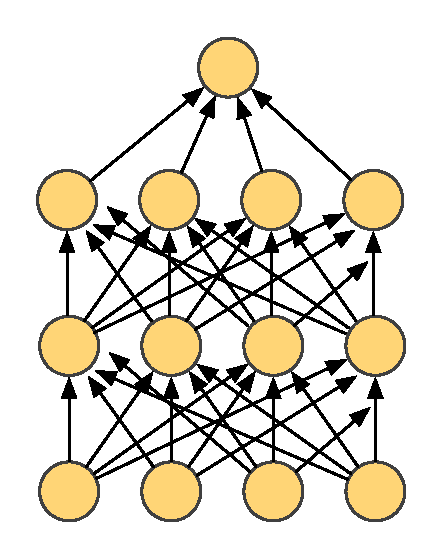
\includegraphics[scale=0.625,angle=270]{figs/nn.eps}	
		\caption{Exemplo de uma arquitetura multi-camadas de uma Rede Neural.}
		\label{f.nn}
	\end{figure}
\end{frame}

\begin{frame}
	\begin{figure}
		\centering
		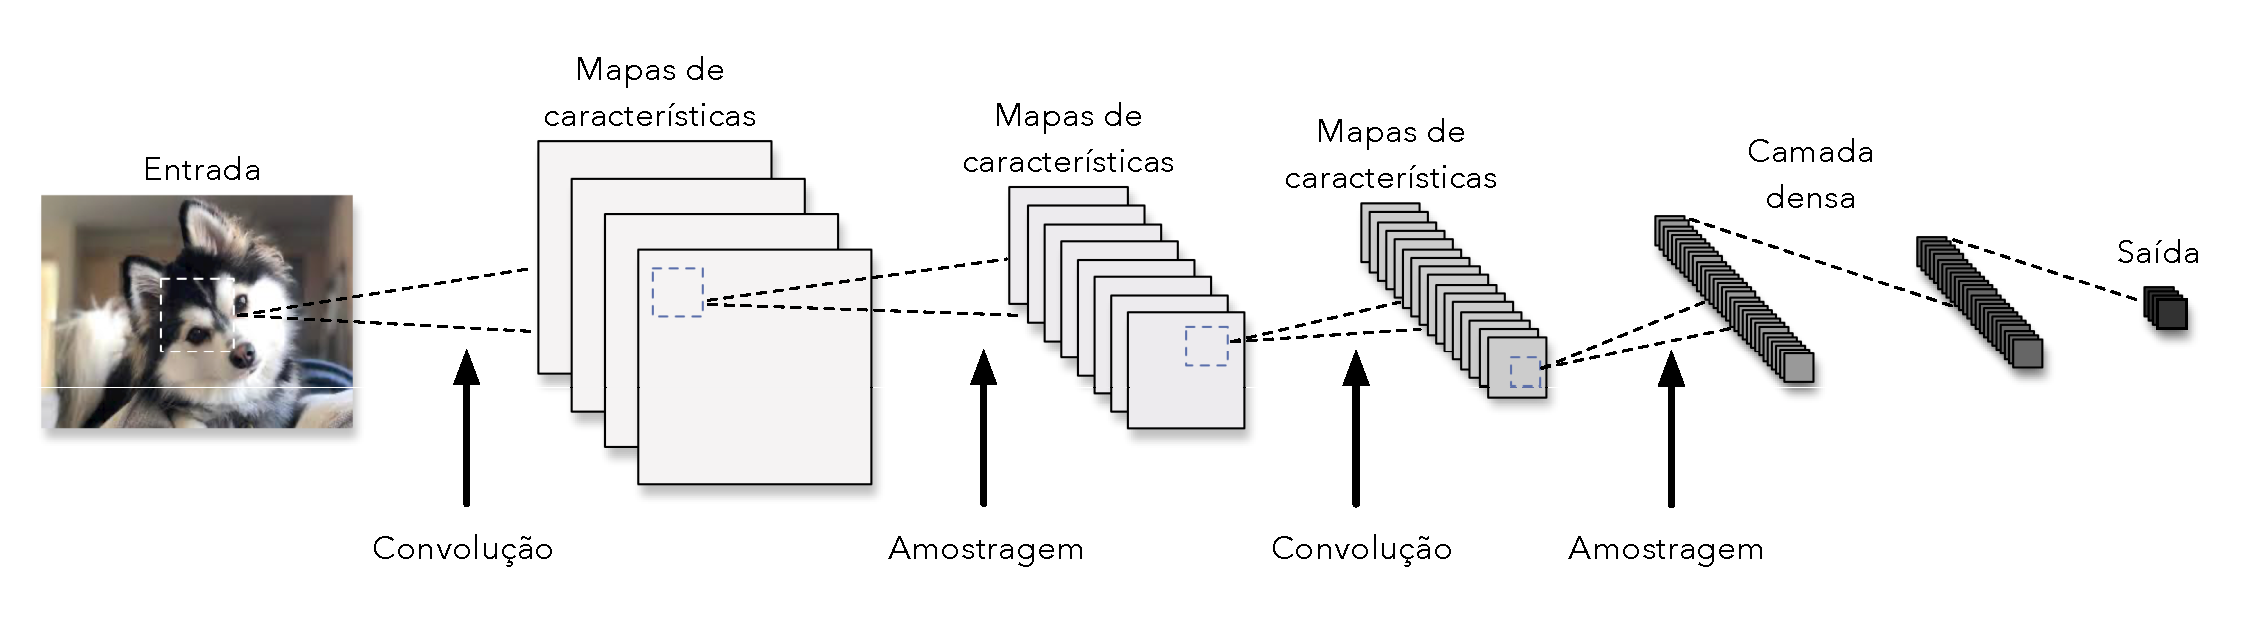
\includegraphics[scale=0.275]{figs/cnn.eps}	
		\caption{Exemplo de uma arquitetura de uma Rede Neural Convolucional.}
		\label{f.cnn}
	\end{figure}
\end{frame}

\begin{frame}
	\vspace*{0.5cm}
	\begin{figure}
		\centering
		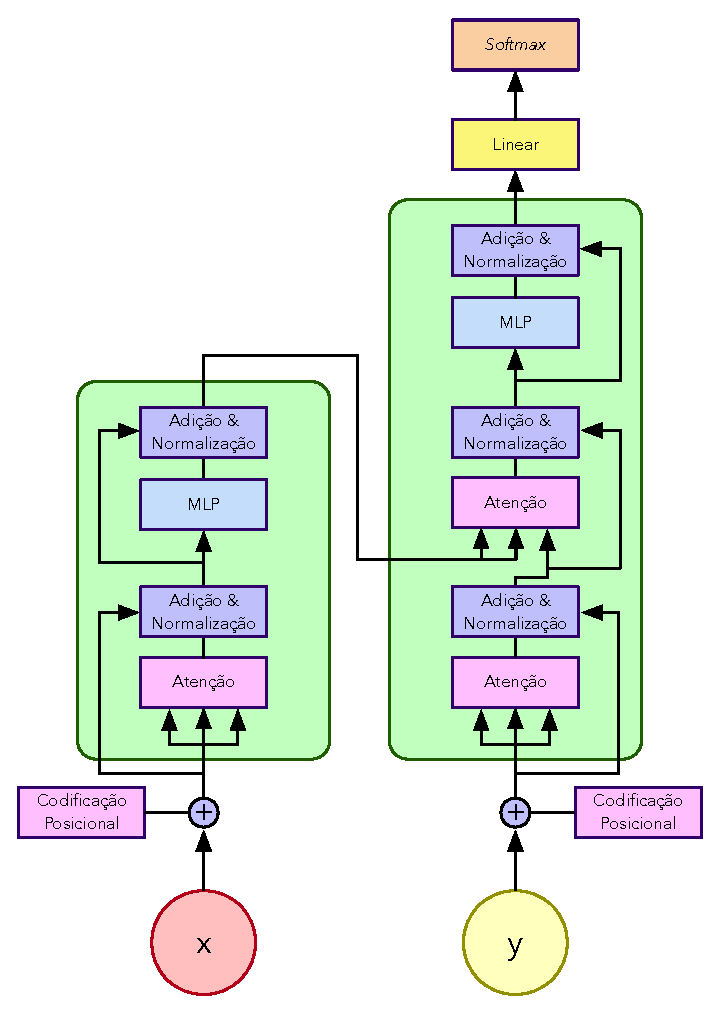
\includegraphics[scale=0.425]{figs/transformer.eps}	
		\caption{Exemplo de uma arquitetura de um Transformador.}
		\label{f.transformer}
	\end{figure}
\end{frame}
\section{Otimização}
\label{s.optimization}

\begin{frame}{Otimização}
	\begin{itemize}
		\justifying
		\item O estudo da otimização~\cite{bertsekas99} possibilita um maior \textbf{conhecimento} sobre o problema;
		\\~\\
		\item \textbf{Otimizar} é encontrar um \textbf{conjunto de variáveis} adequadas para a resolução de um problema.
		\end{itemize}
\end{frame}

\begin{frame}
	\begin{figure}
		\centering
		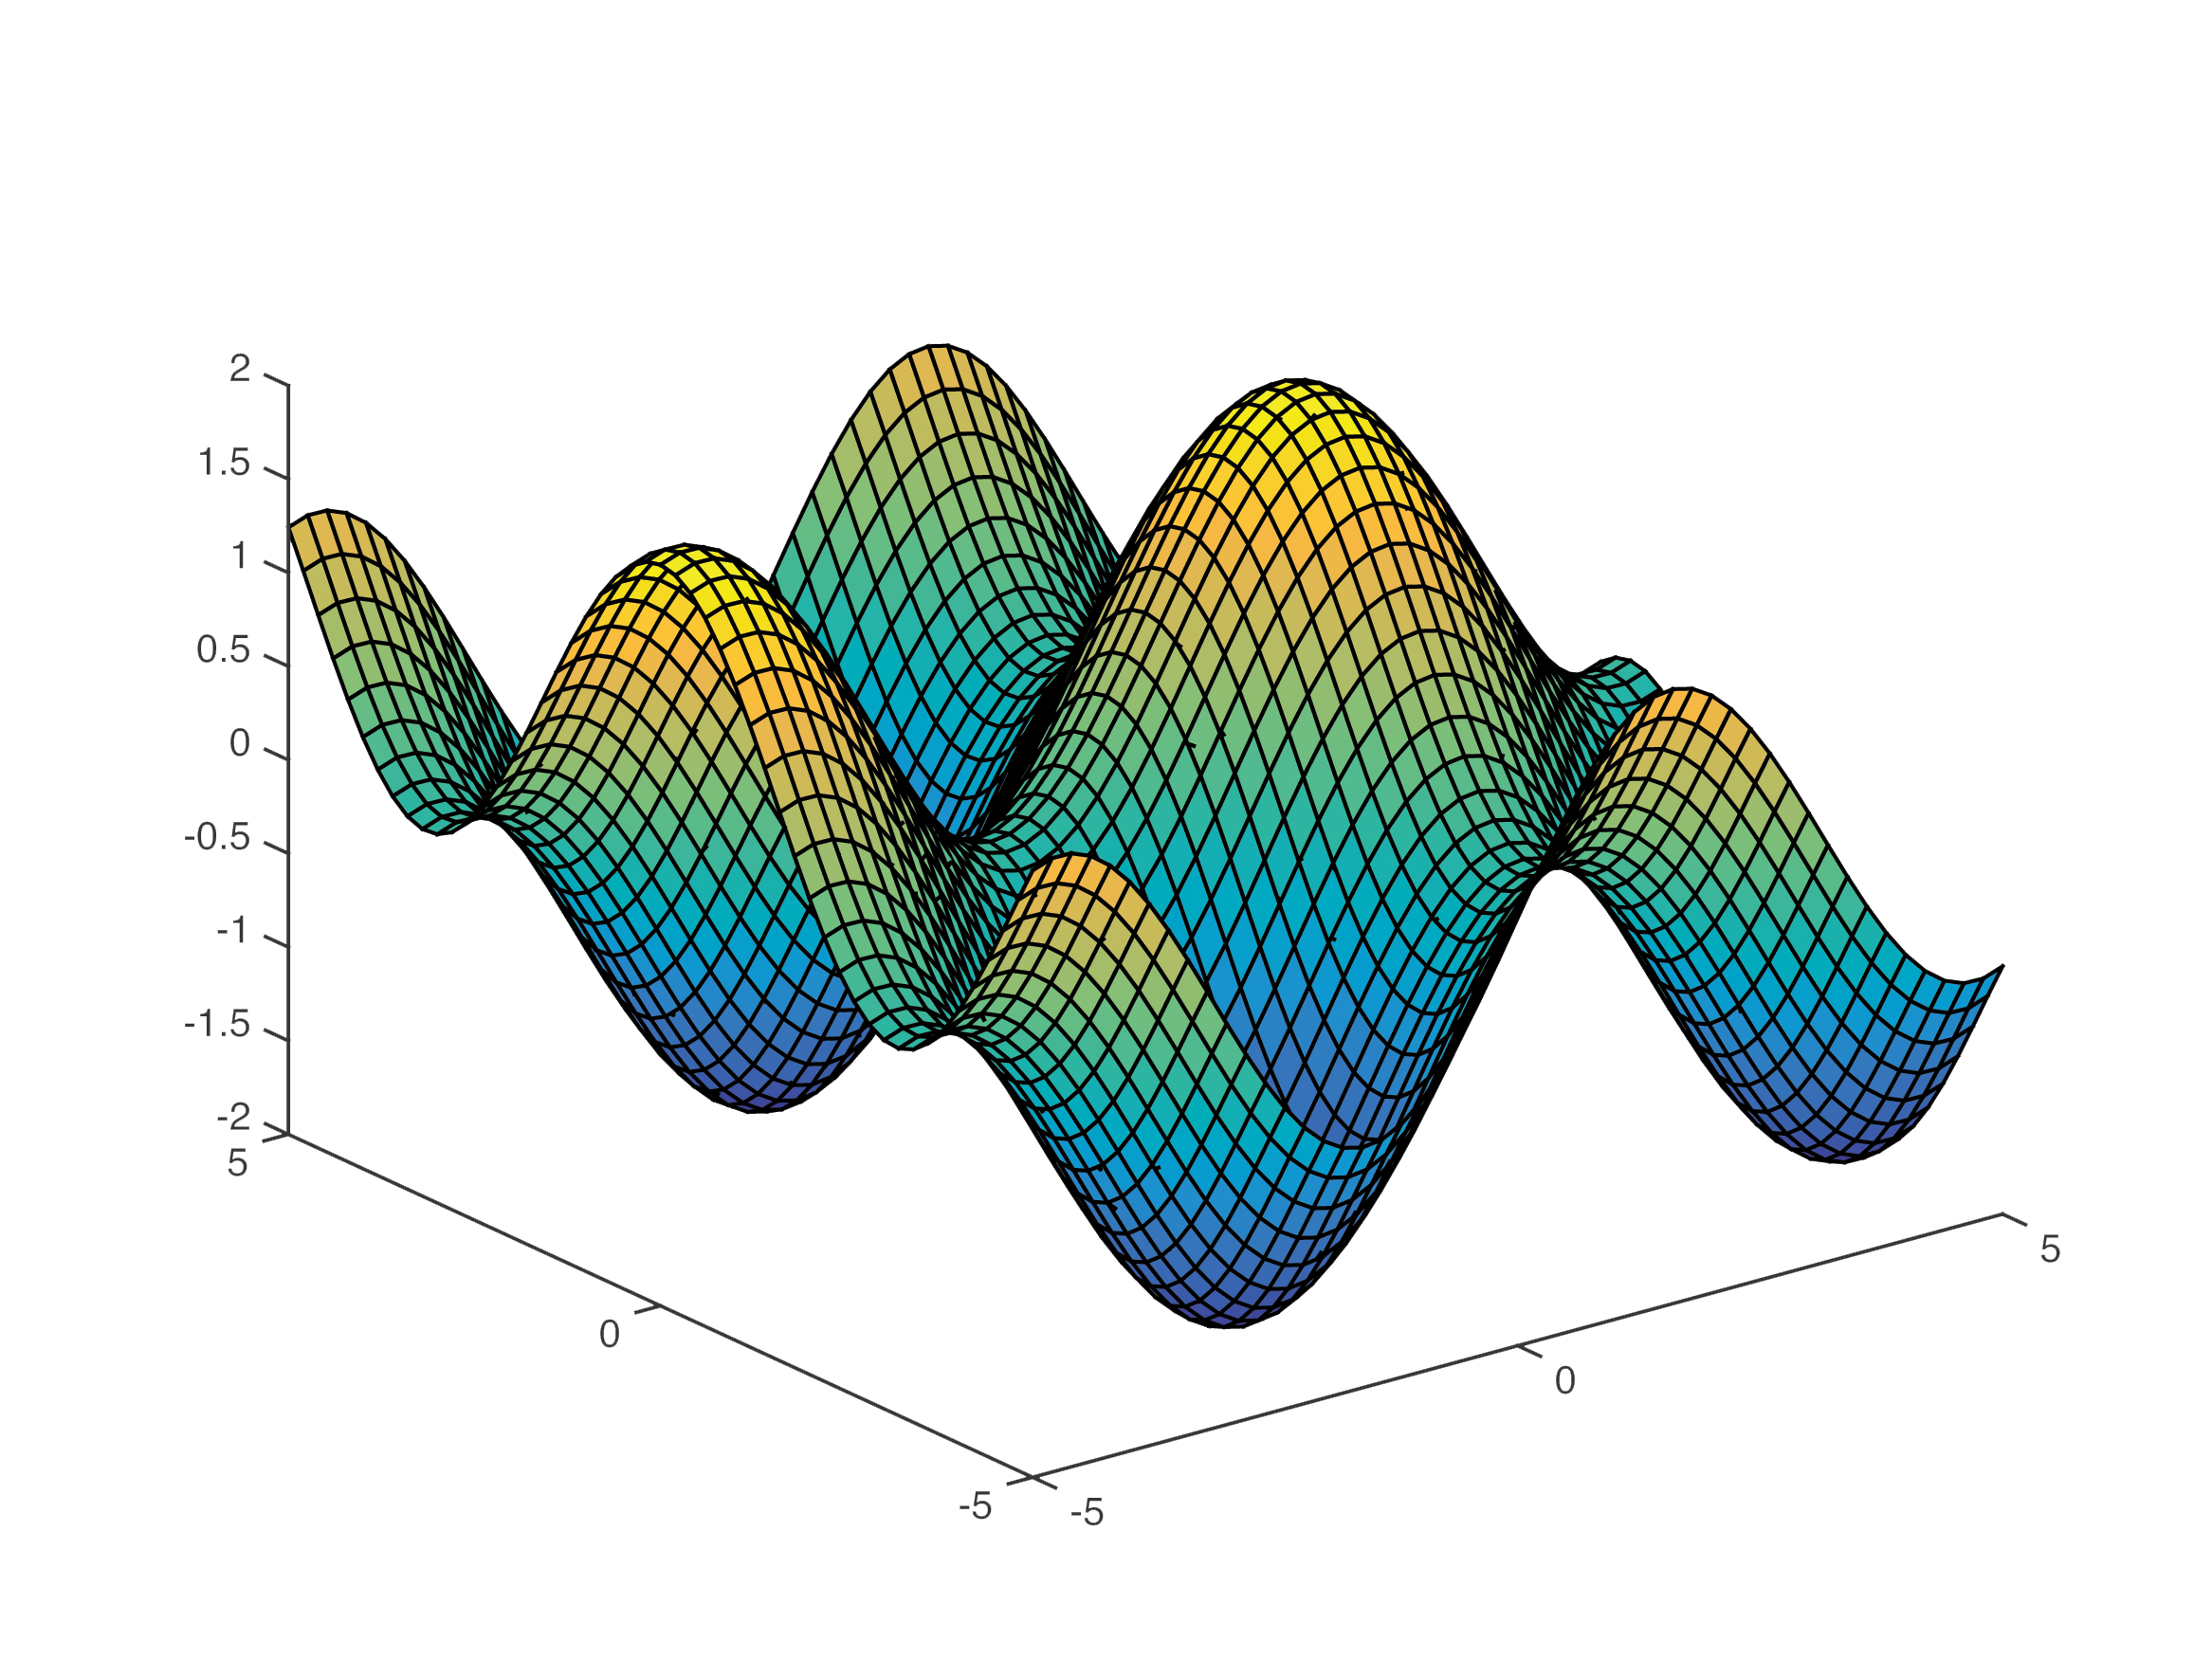
\includegraphics[scale=0.45]{figs/opt_function.png}	
		\caption{Exemplo de superfície da função $f(x,y)=sen(x)+cos(y)$.}
		\label{f.opt_function}
	\end{figure}
\end{frame}

\begin{frame}
	\begin{itemize}
		\justifying
		\item \textbf{Algoritmos} de Aprendizado de Máquina são usualmente \textbf{treinados} através de um processo de \textbf{otimização}~\cite{Lan:20};
		\\~\\
		\item Otimização permite o \textbf{ajuste de parâmetros} (variáveis) de acordo com o problema (\textbf{função de perda});
	\end{itemize}
\end{frame}

\begin{frame}
	\begin{figure}
		\centering
		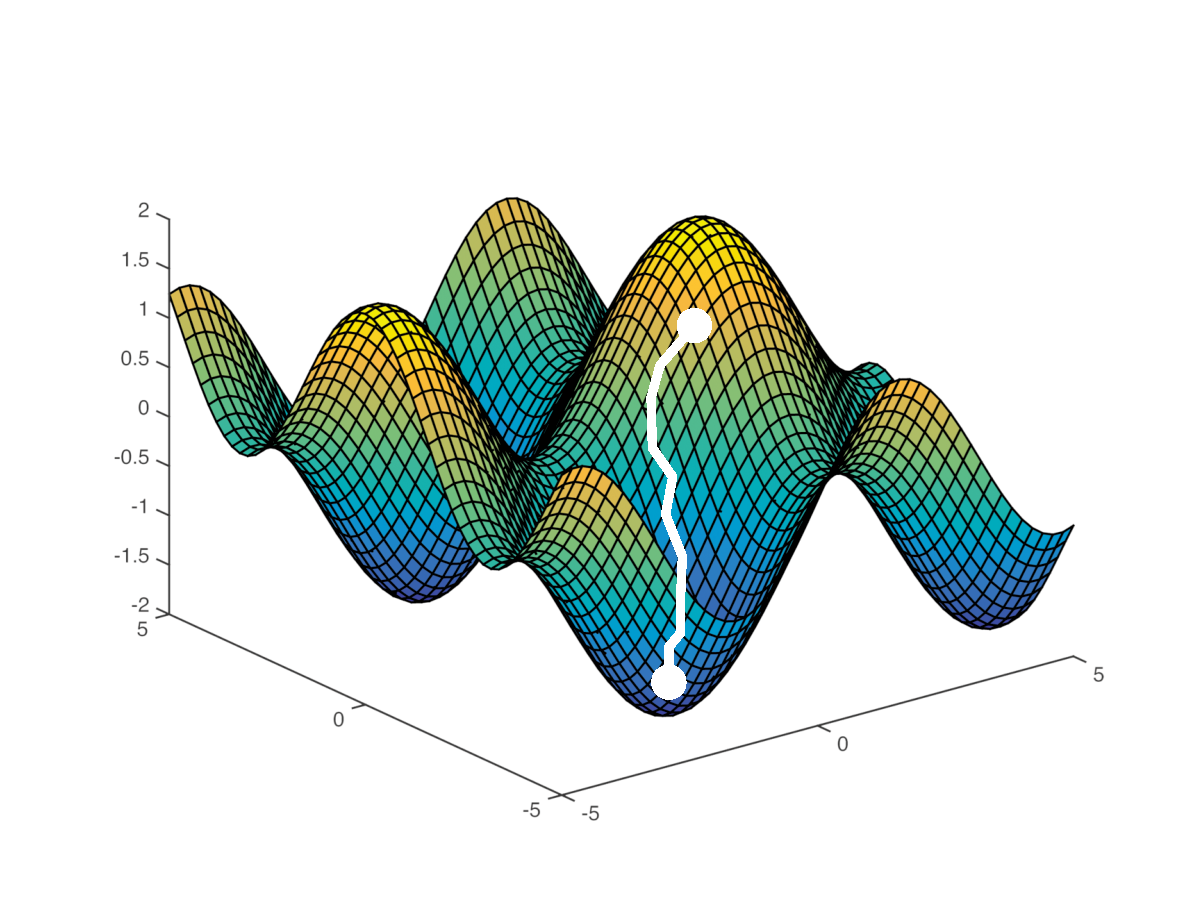
\includegraphics[scale=0.45]{figs/opt_function_opt.eps}	
		\caption{Caminho realizado pelos passos da otimização até o encontro de um ponto de mínimo local.}
		\label{f.opt_function_opt}
	\end{figure}
\end{frame}

\subsection{Otimização Meta-Heurística}
\label{ss.optimization_mh}

\begin{frame}{Otimização Meta-Heurística}
	\begin{itemize}
		\justifying
		\item Modelagem matemática de \textbf{fenômenos da natureza} em algoritmos de \textbf{otimização}~\cite{yang_review};
		\\~\\
		\item \textbf{Heurísticas} (buscas) de \textbf{soluções} em espaços $n$-dimensionais;
		\\~\\
	\end{itemize}
	\vspace*{0.5cm}
	\begin{block}{}
		\centering
		\textbf{Diversificação} x \textbf{Intensificação}
	\end{block}	
\end{frame}
\section{Exemplos de Aplicações}
\label{s.applications}

\begin{frame}{Exemplos de Aplicações}
	\justifying
	A otimização meta-heurística possui uma vasta gama de aplicações, tais como:
	\\~\\
	\begin{itemize}
		\justifying
		\item Otimização de funções matemáticas;
		\\~\\
		\item Otimização de hiperparâmetros;
		\\~\\
		\item Seleção de características;
		\\~\\
		\item \sout{Seleção de modelos}.
	\end{itemize}
\end{frame}

\begin{frame}
	\justifying
	A implementação deste mini-curso está disponível no GitHub\footnote{\url{https://github.com/gugarosa/mh_deep_application}} e utiliza as seguintes bibliotecas:
	\\~\\
	\begin{itemize}
		\justifying
		\item Opytimizer\footnote{\url{https://github.com/gugarosa/opytimizer}};
		\\~\\
		\item Scikit-learn\footnote{\url{https://scikit-learn.org}};
		\\~\\
		\item PyTorch\footnote{\url{https://pytorch.org}}.
	\end{itemize}
\end{frame}


\subsection{Otimização de Funções Matemáticas}
\label{ss.applications_benchmark}

\begin{frame}{Otimização de Funções Matemáticas}
	\begin{figure}
		\centering
		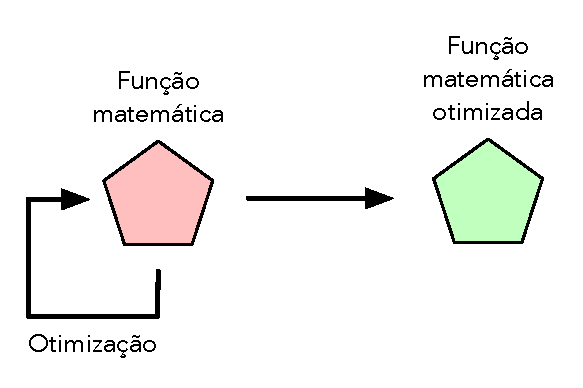
\includegraphics[scale=0.6]{figs/benchmark_opt.eps}	
		\caption{Fluxograma do processo de otimização de funções matemáticas.}
		\label{f.benchmark_opt}
	\end{figure}
	Códigos: \url{https://github.com/gugarosa/mh_deep_application/tree/main/applications/meta_heuristic}
\end{frame}

\subsection{Otimização de Hiperparâmetros}
\label{ss.applications_hyperparameter}

\begin{frame}{Otimização de Hiperparâmetros}
	\begin{figure}
		\centering
		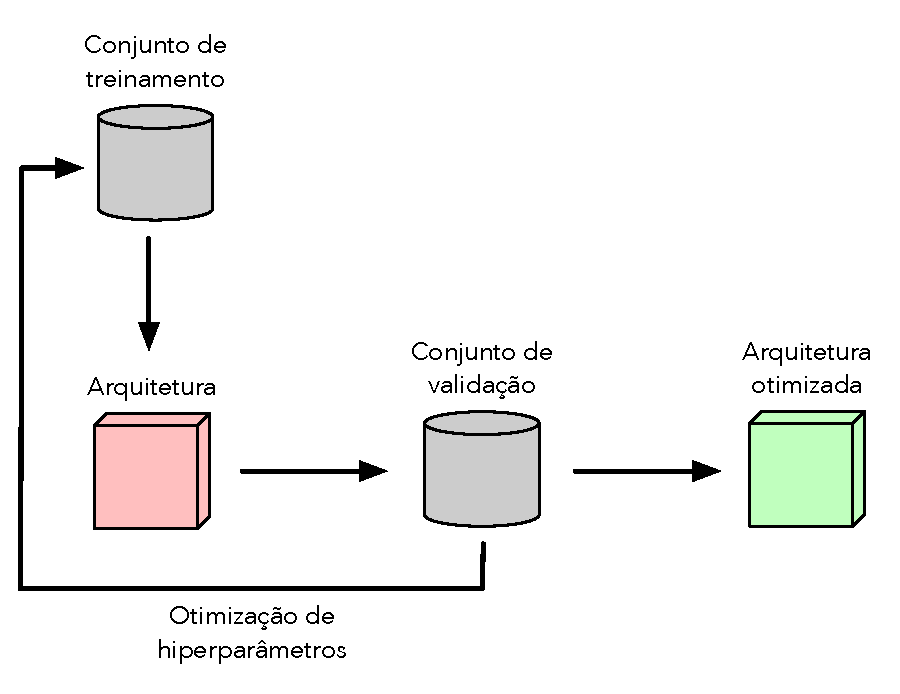
\includegraphics[scale=0.45]{figs/hyperparameter_opt.eps}	
		\caption{Fluxograma do processo de otimização de hiperparâmetros.}
		\label{f.hyperparameter_opt}
	\end{figure}
	Códigos: \url{https://github.com/gugarosa/mh_deep_application/tree/main/applications/hyperparameter_optimization}
\end{frame}

\subsection{Seleção de Características}
\label{ss.applications_feature_selection}

\begin{frame}{Seleção de Características}
	\begin{figure}
		\centering
		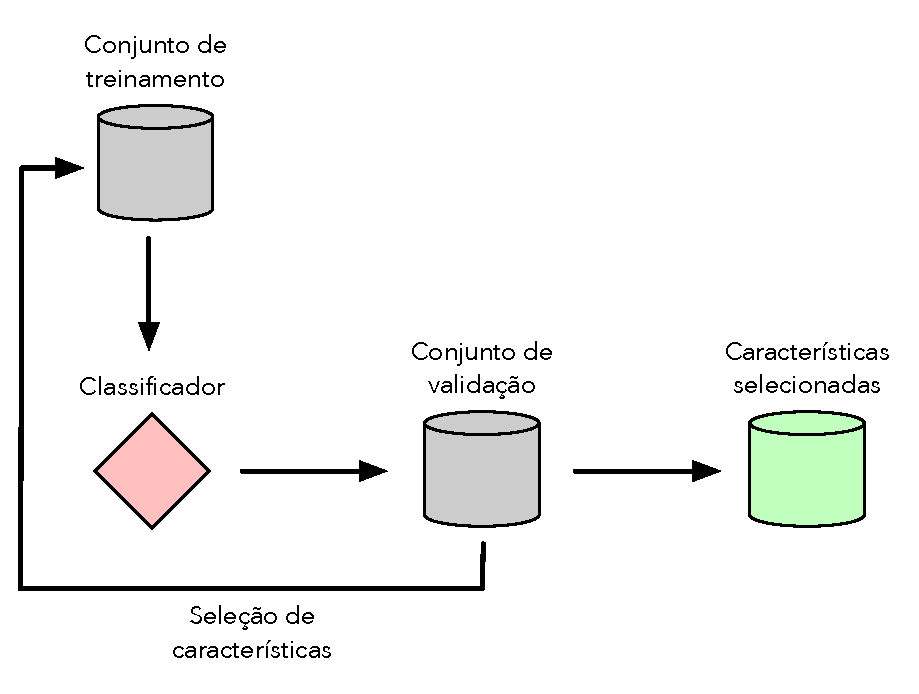
\includegraphics[scale=0.45]{figs/feature_selection.eps}	
		\caption{Fluxograma do processo de seleção de características.}
		\label{f.feature_selection}
	\end{figure}
	Códigos: \url{https://github.com/gugarosa/mh_deep_application/tree/main/applications/feature_selection}
\end{frame}
\section{Conclusão}
\label{s.conclusion}

\begin{frame}{Conclusão}
\end{frame}

% Defines the references and its slides
\section*{Referências}
\begin{frame}[allowframebreaks]
	\bibliography{references}
	\bibliographystyle{unsrt}
\end{frame}

% Defines the standout finishing slide
\begin{frame}[plain,standout]
	\vspace*{2cm}
	Perguntas?
	\\~\\
	Obrigado pela atenção!
	\\~\\
	\begin{figure}[!ht]
		\centering
		
\includegraphics[scale=0.1]{figs/recogna_clear.eps}	
	\end{figure}
\end{frame}

% Ends the document
\end{document}